\documentclass[10pt]{beamer}

\usepackage{etex}
\usepackage{fourier-orns}
\usepackage{ccicons}
\usepackage{amssymb}
\usepackage{amstext}
\usepackage{amsbsy}
\usepackage{amsopn}
\usepackage{amscd}
\usepackage{amsxtra}
\usepackage{amsthm}
\usepackage{float}
\usepackage{color}
\usepackage{mathrsfs}
\usepackage{bm}
\usepackage{lastpage}
\usepackage[nice]{nicefrac}
\usepackage{setspace}
\usepackage{hyperref}
\usepackage{ragged2e}
\usepackage{listings}
\usepackage{algorithms/algorithm}
\usepackage{algorithms/algorithmic}


\usepackage{tikz,pgfplots}
\pgfplotsset{compat=newest}
\usetikzlibrary{patterns, arrows, decorations.pathreplacing, decorations.markings, calc}
\pgfplotsset{plot coordinates/math parser=false}
\newlength\figureheight
\newlength\figurewidth
\usepackage[utf8x]{inputenc}
\usepackage{cancel}
\usepackage{tikz-qtree}

\definecolor{gray}{gray}{0.4}


\setbeamertemplate{footline}{
{\hfill\vspace*{1pt}\href{http://creativecommons.org/licenses/by-sa/3.0/legalcode}{\ccbysa}\hspace{.1cm}
\raisebox{-.075cm}{\href{https://github.com/stepan-a/scalone-2017}{
\includegraphics[scale=.07]{../img/github.png}}}
}\hspace{1cm}}


\setbeamertemplate{navigation symbols}{}
\setbeamertemplate{blocks}[rounded][shadow=true]

\newcommand{\lag}{\mathrm L}
\newcommand{\lead}{\mathrm F}
\newcommand{\Expectation}[1]{\mathbb E \left[#1\right]}
\newcommand{\Variance}[1]{\mathbb E \left[#1\right]}
\newcommand{\ConditionalExpectation}[1]{\mathbb E \left[#1\right]}
\newcommand{\ConditionalVariance}[1]{\mathbb E \left[#1\right]}


\begin{document}

\title{Comments on\\``Estimating Non-Linear DSGEs with ABC...''\\ by Valerio Scalone}
\author{Stéphane Adjemian\footnote{Université du Maine}}
\date{June, 2017}


\begin{frame}
  \maketitle
\end{frame}


\begin{frame}[c]
\frametitle{Estimation of nonlinear DSGE}
\framesubtitle{Reduced form}

  
\[
  \begin{split}
    y_t &= \mathcal M_{\theta, \Sigma} (s_t)+ \eta_t\\
    s_t &= \mathcal S_{\theta,\Sigma}(s_{t-1}, \varepsilon_t)\\
    \varepsilon_t &\underset{\mathrm{iid}}{\sim} \mathcal N \left(\mathbf 0, \Sigma\right)
  \end{split}
\]

\end{frame}


\begin{frame}
\frametitle{Estimation of nonlinear DSGE}
\framesubtitle{Different approaches}

\bigskip
\bigskip
  
\begin{itemize}
\item Most common approach: Forget about nonlinearities!\newline
  \bigskip
\item Take nonlinearity seriously $\Rightarrow$ Nonlinear filters (with lots of particles).\newline
  \bigskip
\item Abandon the land of full information inference (select moments to be matched).
\end{itemize}

\end{frame}


\begin{frame}
\frametitle{Estimation of nonlinear DSGE}
\framesubtitle{Likelihood based approach}

\begin{itemize}
\item In principle, the likelihood (the joint density of the sample) can be expressed as a product of conditional densities and a marginal density for the first observation:
  \[
    \mathcal L(\theta,\Sigma; \mathcal Y_T) = p(y_1|s_0, \theta, \Sigma)p(s_0, \theta, \Sigma)\prod_{t=2}^Tp(y_t|\mathcal Y_{t-1}, \theta, \Sigma)
  \]
  \bigskip
\item But high dimensional integration problems:
  \[
    p(y_t|\mathcal Y_{t-1}, \theta, \Sigma) = \int p(y_t|s_t, \theta, \Sigma)p(s_t|\mathcal Y_{t-1})\mathrm ds
  \]
  \begin{subequations}
    \begin{equation}
      \tag{Prediction}
      p(s_t|\mathcal Y_{t-1}) = \int p(s_t|s_{t-1},\theta,\Sigma)p(s_{t-1}|\mathcal Y_{t-1})\mathrm ds
    \end{equation}
    \begin{equation}
      \tag{Update, Bayes}
      p(s_{t}|\mathcal Y_{t}) \propto p(y_t|s_t,\theta,\Sigma)p(y_t|\mathcal Y_{t-1})
    \end{equation}
  \end{subequations}

\end{itemize}
\end{frame}


\begin{frame}
\frametitle{Estimation of nonlinear DSGE}
\framesubtitle{Issues with likelihood based approach}

\bigskip
\bigskip
  
\begin{itemize}

\item Evaluation of the high dimensional integrals:\newline

  \begin{itemize}
  \item Monte Carlo,
  \item Numerical approximations (quadrature, cubature, ...)
  \end{itemize}

  \bigskip

\item Resampling $\Rightarrow$ Non differentiability.\newline

  \bigskip

\item Measurement errors are mandatory.\newline

  \bigskip
  
\item Choice for the initial condition.
  
\end{itemize}

\end{frame}

\begin{frame}
\frametitle{Likelihood cross sections}
\framesubtitle{RBC model}

\begin{figure}[H]
   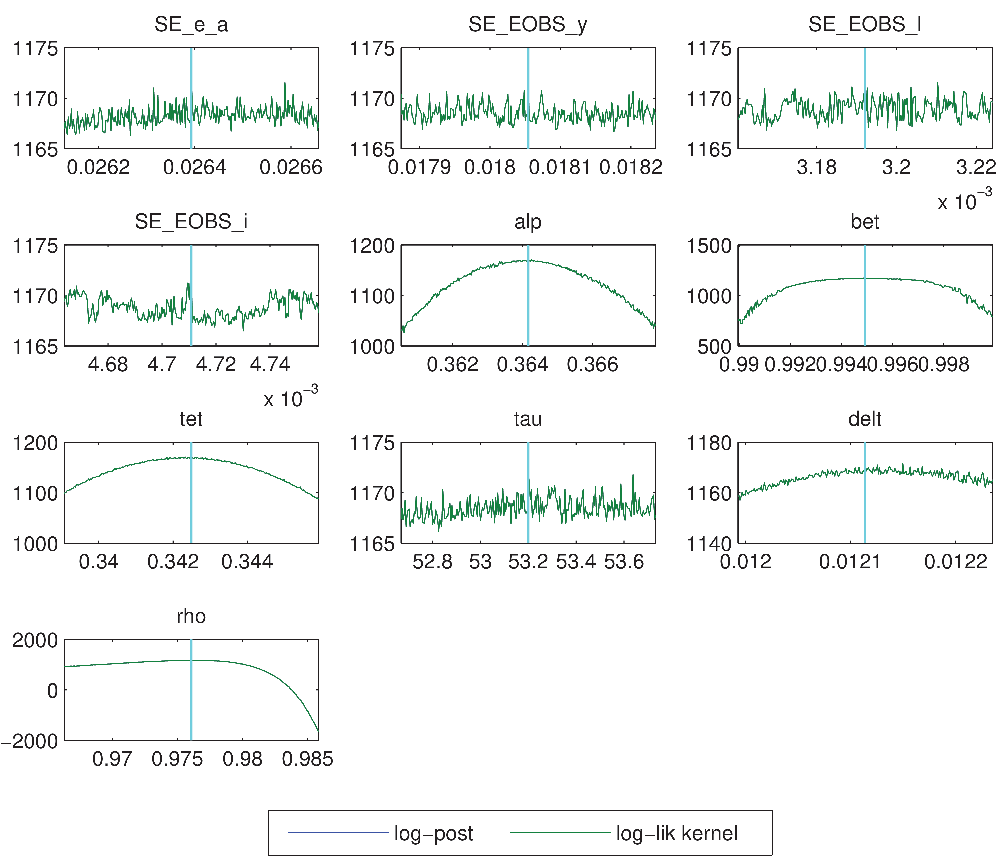
\includegraphics[scale=.6]{../img/SIR_likelihood_cross_sections.pdf}
 \end{figure}
 
\end{frame}


\begin{frame}
  \frametitle{Posterior marginals}
\framesubtitle{RBC model}

\begin{figure}[H]
   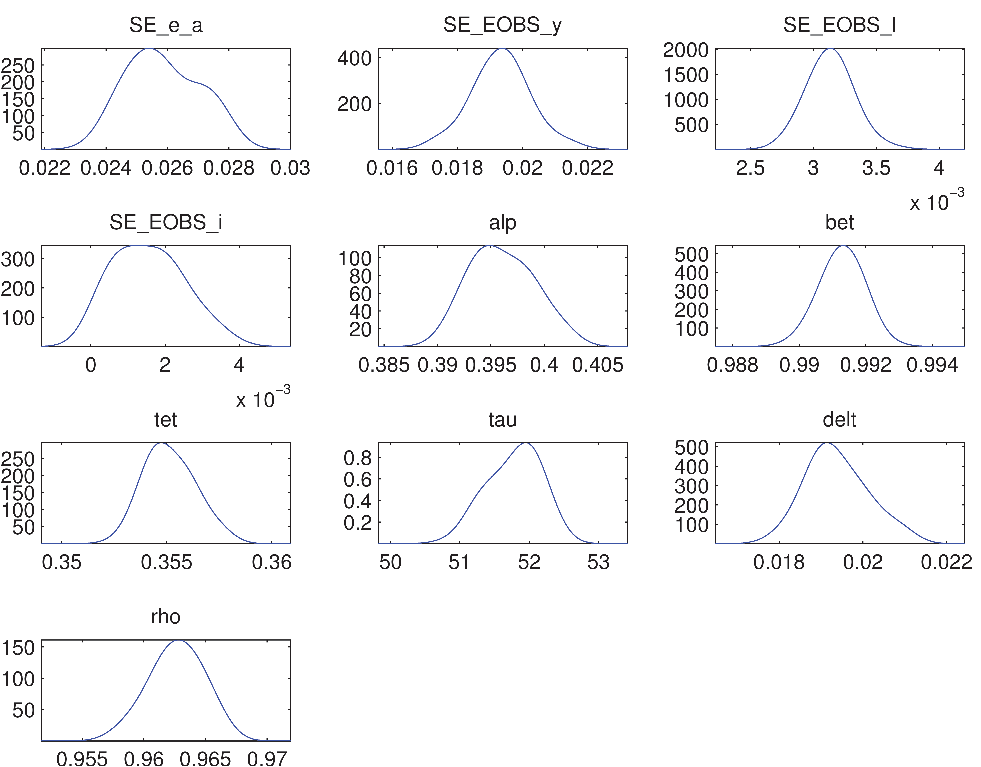
\includegraphics[scale=.5]{../img/SIR_posterior_marginals.pdf}
 \end{figure}
 
\end{frame}


\begin{frame}
  \frametitle{Conditional likelihood?}

  \begin{itemize}
  \item No measurement errors and $\sharp\{y_t\}=\sharp\{\varepsilon_t\}$
    \[
      y_t = \mathcal F_{\theta,\Sigma} \left(s_{t-1}, \varepsilon_t\right) \triangleq \mathcal M_{\theta,\Sigma}\left(\mathcal S_{\theta,\Sigma}(s_{t-1}, \varepsilon_t)\right)
    \]
    
    \bigskip

  \item Assume that $\mathcal F$ is bijective w.r.t. the second argument.

    \bigskip

  \item Given $s_0$ (the non stochastic steady state) and $y_1$ (observed) we deduce $\varepsilon_1$ and update the state: $s_1$.\newline

    $\Rightarrow$ We can then recursively deduce the sequence $\{\varepsilon_t\}_{t=1}^T$ from the sample and a given initial condition for the states.\newline

    \bigskip

  \item If the innovations are Gaussian, the likelihood is defined by:
    \[
      \mathcal L(\theta, \Sigma; \mathcal Y_T, s_0) = (2\pi)^{-\frac{T}{2}}|\Sigma|^{-\frac{1}{2}}e^{-\frac{1}{2}\sum_{t=1}^T \varepsilon_t'\Sigma^{-1}\varepsilon_t}
    \]

    \bigskip

    Note that $s_0$ could be added to the set of estimated parameters.

  \end{itemize}
\end{frame}


\begin{frame}
  \frametitle{ABC}
  \framesubtitle{paths}

  \begin{itemize}

  \item Posterior is:
    \[
      p(\theta,\Sigma|\mathcal Y_T) \propto \mathcal L (\theta,\Sigma; \mathcal Y_T) p(\theta,\Sigma)
    \]

    \bigskip
    
  \item ABC replaces the (intractable) likelihood with a distance between simulated paths ($\mathcal Y_T^\star(\theta,\Sigma)$) and actual paths ($\mathcal Y_T$).\newline

    \bigskip
    
  \item Basic sampling scheme:
    \begin{itemize}
    \item Sample $\theta$ from the prior distribution.
    \item Accept the draw if $||\mathcal Y_T^\star(\theta,\Sigma)-\mathcal Y_T||<\varepsilon$.
    \end{itemize}

    \bigskip

  \item But the probability of accepting a draw tends rapidly to zero
    when the number of observed variables or the number of
    observations grows. Because the volume of the hyper-cube where the
    sample lives grows exponentially (curse of dimensionality).

    \bigskip
    
  \item Asymptotics? Choice of the norm?
    
  \end{itemize}
\end{frame}


\begin{frame}
  \frametitle{ABC}
  \framesubtitle{moments}

  \begin{itemize}

  \item To overcome the curse of dimensionality, we can compare moments instead of paths.\newline

  \item We now accept the draws from the prior distribution if:
    \[
      ||m\left(\mathcal Y_T^\star(\theta,\Sigma)\right)-m(\mathcal Y_T)||<\varepsilon
    \]
    
  \item \textsc{Intuition} if the vector $m$ contains the sufficient
    statistics w.r.t. $\theta$ and $\Sigma$, this should lead to the
    same inference than the expression of the posterior based on
    the likelihood.\newline

  \item But
    \begin{itemize}
    \item Has this been proven?
    \item Find sufficient statistics for AR(p) or linear models is easy. 
    \item What about the sufficient statistics for DSGE models?
    \item How do we find them?
    \item Is the set of sufficient statistics finite?
    \end{itemize}
    
  \end{itemize}
\end{frame}


\begin{frame}
  \frametitle{ABC}
  \framesubtitle{A non parametric method of simulated  moments, I}

  \bigskip
  
  \begin{itemize}
    
  \item If we forget the issue with the choice of the sufficient
    statistics, the ABC is motivated as a non parametric Bayesian
    method of moments.\newline

    \bigskip

  \item Close to what is done in recent Christiano \textit{et al.}
    papers, except that the normality of the moments is not
    imposed. An assumption clearly too strong for finite samples (as
    illustrated with the AR(1) example).\newline

  \end{itemize}

  \bigskip
  
  \[
    p(\theta,\Sigma|\mathcal Y_T) \widetilde{\propto}
    (2\pi)^{-\frac{n}{2}}|\widehat V|^{-\frac{1}{2}}e^{-\frac{n}{2}\left(m\left(\mathcal Y_T^{\star}(\theta,\Sigma)\right)-m\left(\mathcal Y_T\right)\right)'\widehat V^{-1}\left(m\left(\mathcal Y_T^{\star}(\theta,\Sigma)\right)-m\left(\mathcal Y_T\right)\right)}p(\theta,\Sigma)
  \]


\end{frame}

\begin{frame}
  \frametitle{ABC}
  \framesubtitle{A non parametric method of simulated  moments, II}

  \bigskip
  
  \begin{itemize}
    
  \item Cannot we interpret the Gaussian approximation made by
    Christiano \textit{et al.} as a choice for a particular kernel?\dots\newline

  \item \dots\ If I use the ABC-kernel-MCMC approach with a Gaussian
    kernel (not described in the paper ), I expect to have results
    very similar to Christiano \textit{et al.}.\newline

  \item The choice of the bandwidth parameter of the kernel is not
    discussed in the paper, though it seems equivalent to the choice of the
    long run (co)variance in Christiano \emph{et al.}\newline

  \item The choice for $\epsilon$ also implicitly pins down the weight of
    the likelihood approximation relative to the prior. The larger
    $\epsilon$ is the closer are the posterior and prior
    distributions.

  \end{itemize}
\end{frame}



\begin{frame}
  \frametitle{More remarks on the paper}
  \framesubtitle{Comparison}

  \begin{itemize}

  \item ABC, BLI and likelihood based are compared in section 4.
    
  \item AR(1) and RBC models are considered.

  \item The set of moments is not always clear.

  \item For the RBC model, the set of moments is probably too
    small. The reduced form solution is a VARMA(2,1) but only first
    order auto covariance is used.

  \item Why not to compare the posterior distributions more seriously?
    \emph{ie} test if the posterior densities or cumulated distribution
    functions are significantly different.

  \item Given the title of the paper, we expect a comparison with a
    non approximated DSGE model (with non linear filters to evaluate
    the likelihood).

  \item Only covariances are used to estimate the NK-ZLB model. Worse
    than in the case of the RBC model. It is not possible to capture
    the nonlinearity non normality with these moments.
    
  \end{itemize}
\end{frame}



\end{document}

% Local Variables:
% ispell-check-comments: exclusive
% ispell-local-dictionary: "british"
% End: